\documentclass[../../main.tex]{subfiles}

\begin{document}

\section{Optimización}

%==================================================
% INTRODUCCIÓN
%==================================================

\subsection{Formulación de problemas de optimización}

\begin{frame}{Optimizar es elegir la mejor alternativa factible}
\begin{itemize}
  \item La optimización determina los valores de las variables de decisión que minimizan o maximizan una función objetivo.
  \item En ingeniería, el objetivo suele representar costo, energía, masa, tiempo, error, eficiencia o potencia.
  \item Las restricciones expresan límites físicos, económicos, ambientales o de seguridad.
\end{itemize}

\[
\boxed{
\min_{\mathbf{x}}\; f(\mathbf{x})
\quad \text{sujeto a} \quad
g_i(\mathbf{x})\le 0,
\qquad
h_j(\mathbf{x})=0
}
\]

\begin{block}{Idea central}
Una solución útil no solo debe mejorar el objetivo: también debe ser factible.
\end{block}
\end{frame}

\begin{frame}{Raíces y óptimos responden preguntas diferentes}
\begin{columns}[T]
\begin{column}{0.48\textwidth}
\textbf{Localización de raíces}
\[
f(x)=0
\]
\begin{itemize}
  \item Busca cruces con el eje horizontal.
  \item Puede usar bisección, Newton o secante.
  \item El signo de la función ayuda a encerrar una raíz.
\end{itemize}
\end{column}

\begin{column}{0.48\textwidth}
\textbf{Optimización}
\[
\min f(x)
\quad \text{o} \quad
\max f(x)
\]
\begin{itemize}
  \item Busca el mejor valor de la función.
  \item Compara alturas, no solamente signos.
  \item Puede incluir restricciones y varias variables.
\end{itemize}
\end{column}
\end{columns}

\begin{alertblock}{Relación}
Si el óptimo es interior y $f$ es diferenciable, una condición necesaria es $f'(x^*)=0$.
\end{alertblock}
\end{frame}

\begin{frame}{Las derivadas clasifican puntos estacionarios}
Sea $x^*$ un punto interior con
\[
f'(x^*)=0.
\]

\begin{columns}[T]
\begin{column}{0.31\textwidth}
\begin{block}{Mínimo local}
\[
f''(x^*)>0
\]
La curva es convexa cerca de $x^*$.
\end{block}
\end{column}

\begin{column}{0.31\textwidth}
\begin{block}{Máximo local}
\[
f''(x^*)<0
\]
La curva es cóncava cerca de $x^*$.
\end{block}
\end{column}

\begin{column}{0.31\textwidth}
\begin{block}{Prueba inconclusa}
\[
f''(x^*)=0
\]
Se requieren otros argumentos.
\end{block}
\end{column}
\end{columns}

\medskip
Los óptimos también pueden aparecer en la frontera o en puntos donde la función no es diferenciable.
\end{frame}

\begin{frame}{La forma del problema determina el método}
\small
\begin{tabular}{p{0.27\textwidth}p{0.30\textwidth}p{0.34\textwidth}}
\toprule
\textbf{Clasificación} & \textbf{Característica} & \textbf{Métodos frecuentes}\\
\midrule
Unidimensional & Una variable de decisión & Sección dorada, interpolación parabólica, Newton, Brent\\
Multidimensional & Dos o más variables & Búsqueda de patrones, descenso, Newton, cuasi-Newton\\
Sin restricciones & Toda $\mathbf{x}$ admisible pertenece al dominio & Métodos directos o con gradiente\\
Con restricciones & Igualdades, desigualdades o cotas & Programación lineal, penalización, multiplicadores, SQP\\
Variables enteras & Algunas decisiones son discretas & Enumeración, ramificación y acotamiento, métodos mixtos\\
\bottomrule
\end{tabular}
\end{frame}

%==================================================
% OPTIMIZACIÓN UNIDIMENSIONAL
%==================================================

\subsection{Optimización unidimensional sin restricciones}

\begin{frame}{Un intervalo unimodal permite encerrar un óptimo}
Una función es \textbf{unimodal} en $[x_l,x_u]$ si contiene un solo mínimo o un solo máximo local en ese intervalo.

\begin{center}
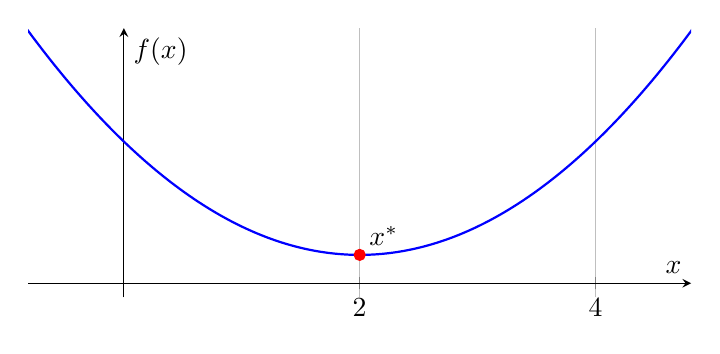
\begin{tikzpicture}
\begin{axis}[
  width=10cm,height=5cm,
  domain=-1:5,samples=160,
  axis lines=middle,
  xlabel={$x$},ylabel={$f(x)$},
  xtick={0,2,4},ytick=\empty,
  ymin=-0.5,ymax=9,
  grid=major
]
\addplot[blue,thick] {(x-2)^2+1};
\addplot[only marks,mark=*,red] coordinates {(2,1)};
\node[above right] at (axis cs:2,1) {$x^*$};
\end{axis}
\end{tikzpicture}
\end{center}

La unimodalidad es esencial para descartar regiones sin perder el óptimo buscado.
\end{frame}

\subsubsection{Búsqueda de la sección dorada}

\begin{frame}{La sección dorada reutiliza una evaluación}
La razón dorada usada por Chapra es
\[
R=\frac{\sqrt{5}-1}{2}\approx0.618034.
\]

Para el intervalo $[x_l,x_u]$ se definen dos puntos interiores:
\[
x_1=x_l+R(x_u-x_l),
\qquad
x_2=x_u-R(x_u-x_l).
\]

\begin{itemize}
  \item Se comparan $f(x_1)$ y $f(x_2)$.
  \item Se elimina la región que no contiene el óptimo.
  \item En la siguiente iteración uno de los puntos anteriores se reutiliza.
  \item El intervalo se reduce por un factor aproximado de $0.618$ por iteración.
\end{itemize}
\end{frame}

\begin{frame}{Regla de actualización para un mínimo}
Suponga $x_2<x_1$ dentro de $[x_l,x_u]$.

\begin{columns}[T]
\begin{column}{0.47\textwidth}
\begin{block}{Si $f(x_2)<f(x_1)$}
El mínimo está en
\[
[x_l,x_1].
\]
Se actualiza
\[
x_u\leftarrow x_1.
\]
\end{block}
\end{column}

\begin{column}{0.47\textwidth}
\begin{block}{Si $f(x_2)\ge f(x_1)$}
El mínimo está en
\[
[x_2,x_u].
\]
Se actualiza
\[
x_l\leftarrow x_2.
\]
\end{block}
\end{column}
\end{columns}

\medskip
Para localizar un máximo se invierte la comparación o se minimiza $-f(x)$.
\end{frame}

\begin{frame}{La longitud del intervalo controla el error}
Después de $n$ reducciones,
\[
L_n=R^nL_0,
\qquad
L_0=x_u^{(0)}-x_l^{(0)}.
\]

Para exigir $L_n\le L_d$:
\[
\boxed{
n\ge
\frac{\ln(L_d/L_0)}{\ln R}
}
\]

Una estimación relativa empleada como criterio de paro es
\[
\varepsilon_a
\approx
(1-R)\left|\frac{x_u-x_l}{x_{\mathrm{opt}}}\right|100\%.
\]

El criterio basado en el intervalo es especialmente útil cuando no se conoce el óptimo verdadero.
\end{frame}

\begin{frame}{Ejemplo de Chapra: maximizar una función unimodal}
Encontrar el máximo de
\[
f(x)=2\sin x-\frac{x^2}{10},
\qquad 0\le x\le4.
\]

Primera iteración:
\[
x_1=2.4721,
\qquad
x_2=1.5279,
\]
\[
f(x_1)=0.6300,
\qquad
f(x_2)=1.7647.
\]

Como $f(x_2)>f(x_1)$, el máximo queda encerrado en
\[
[0,2.4721].
\]

Después de ocho iteraciones, Chapra obtiene $x\approx1.4427$; el valor de referencia es $x^*\approx1.4276$.
\end{frame}

\begin{frame}{La gráfica confirma el máximo del ejemplo}
\centering
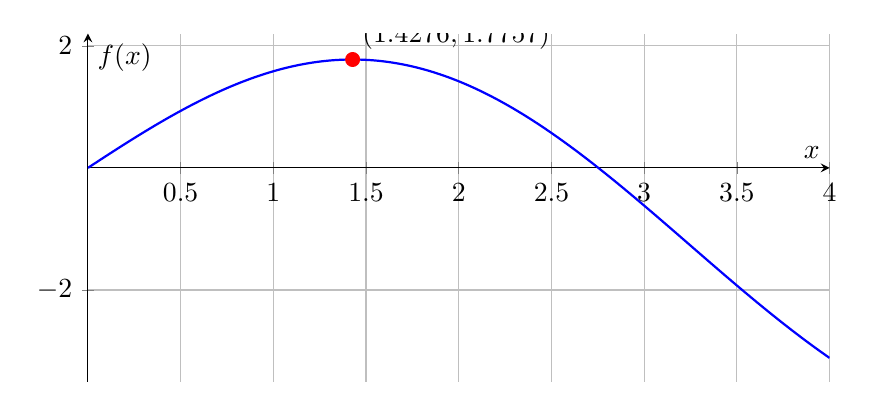
\begin{tikzpicture}
\begin{axis}[
  width=11cm,height=6cm,
  domain=0:4,samples=220,
  axis lines=middle,
  xlabel={$x$},ylabel={$f(x)$},
  grid=major,
  ymin=-3.5,ymax=2.2
]
\addplot[blue,thick] {2*sin(deg(x))-x^2/10};
\addplot[only marks,mark=*,red,mark size=2.5pt] coordinates {(1.4276,1.7757)};
\node[above right] at (axis cs:1.4276,1.7757) {$(1.4276,1.7757)$};
\end{axis}
\end{tikzpicture}
\end{frame}

\begin{frame}[fragile]{Python: búsqueda de la sección dorada}
\scriptsize
\begin{lstlisting}[style=mypython]
def seccion_dorada(f, xl, xu, tol=1e-5, imax=100):
    R = (5**0.5 - 1) / 2
    x1 = xl + R * (xu - xl)
    x2 = xu - R * (xu - xl)
    f1, f2 = f(x1), f(x2)

    for i in range(1, imax + 1):
        if abs(xu - xl) <= tol:
            break
        if f2 < f1:              # minimizacion
            xu, x1, f1 = x1, x2, f2
            x2 = xu - R * (xu - xl)
            f2 = f(x2)
        else:
            xl, x2, f2 = x2, x1, f1
            x1 = xl + R * (xu - xl)
            f1 = f(x1)

    xopt = (xl + xu) / 2
    return xopt, f(xopt), i
\end{lstlisting}
\end{frame}

\subsubsection{Interpolación parabólica}

\begin{frame}{Una parábola aproxima la forma local de la función}
Dados tres puntos $x_0,x_1,x_2$, se interpola una parábola y se toma su vértice como nueva aproximación:

\small
\[
x_3=
\frac{
f_0(x_1^2-x_2^2)+
f_1(x_2^2-x_0^2)+
f_2(x_0^2-x_1^2)
}{
2\left[
f_0(x_1-x_2)+
f_1(x_2-x_0)+
f_2(x_0-x_1)
\right]
},
\]
donde $f_i=f(x_i)$.

\begin{itemize}
  \item Puede converger más rápido que la sección dorada.
  \item No requiere derivadas analíticas.
  \item Puede fallar si los puntos producen un denominador cercano a cero.
  \item Es más confiable cuando se mantiene un intervalo que encierra el óptimo.
\end{itemize}
\end{frame}

\begin{frame}{La interpolación parabólica exige controles numéricos}
Antes de aceptar $x_3$ conviene verificar:
\begin{enumerate}
  \item Los tres valores $x_0,x_1,x_2$ son distintos.
  \item El denominador de la fórmula no es demasiado pequeño.
  \item La nueva aproximación pertenece al intervalo permitido.
  \item La función mejora o el intervalo se reduce.
  \item Existe un máximo de iteraciones y un criterio de paro.
\end{enumerate}

\begin{alertblock}{Práctica recomendada}
Combinar interpolación con una búsqueda cerrada evita que un paso inestable destruya el encerramiento del óptimo.
\end{alertblock}
\end{frame}

\subsubsection{Métodos de Newton y Brent}

\begin{frame}{Newton busca una raíz de la primera derivada}
Al aplicar Newton-Raphson a $f'(x)=0$ se obtiene
\[
\boxed{
x_{i+1}=x_i-\frac{f'(x_i)}{f''(x_i)}
}
\]

\begin{itemize}
  \item Cerca de un óptimo regular puede converger con rapidez cuadrática.
  \item Requiere $f''(x_i)\neq0$.
  \item Una aproximación inicial deficiente puede causar divergencia.
  \item Se debe comprobar el signo de $f''(x^*)$ y comparar con las fronteras.
\end{itemize}

Para derivadas no disponibles analíticamente pueden utilizarse diferencias centrales:
\[
f'(x)\approx\frac{f(x+h)-f(x-h)}{2h},
\qquad
f''(x)\approx\frac{f(x+h)-2f(x)+f(x-h)}{h^2}.
\]
\end{frame}

\begin{frame}[fragile]{Python: Newton para un mínimo unidimensional}
\scriptsize
\begin{lstlisting}[style=mypython]
def newton_opt(df, d2f, x0, tol=1e-8, imax=50):
    x = x0
    for i in range(1, imax + 1):
        curvatura = d2f(x)
        if abs(curvatura) < 1e-12:
            raise ValueError("Segunda derivada casi nula")
        x_nuevo = x - df(x) / curvatura
        if abs(x_nuevo - x) <= tol * max(1, abs(x_nuevo)):
            x = x_nuevo
            break
        x = x_nuevo

    if d2f(x) <= 0:
        raise ValueError("El punto no es un minimo local")
    return x, i
\end{lstlisting}
\end{frame}

\begin{frame}{Brent combina confiabilidad y rapidez}
El método de Brent para optimización alterna entre:
\begin{itemize}
  \item un paso de interpolación parabólica, cuando es seguro y útil;
  \item un paso de sección dorada, cuando la interpolación no es confiable.
\end{itemize}

\begin{center}
\begin{tabular}{lccc}
\toprule
\textbf{Método} & \textbf{Derivadas} & \textbf{Encierra óptimo} & \textbf{Comportamiento}\\
\midrule
Sección dorada & No & Sí & Robusto, lineal\\
Parabólico & No & Opcional & Rápido cerca del óptimo\\
Newton & Sí & No & Muy rápido, sensible\\
Brent & No & Sí & Robusto y eficiente\\
\bottomrule
\end{tabular}
\end{center}
\end{frame}

%==================================================
% OPTIMIZACIÓN MULTIDIMENSIONAL
%==================================================

\subsection{Optimización multidimensional sin restricciones}

\begin{frame}{El gradiente señala el crecimiento más rápido}
Para $f:\mathbb{R}^n\rightarrow\mathbb{R}$,
\[
\nabla f(\mathbf{x})=
\begin{bmatrix}
\partial f/\partial x_1\\
\vdots\\
\partial f/\partial x_n
\end{bmatrix}.
\]

\begin{itemize}
  \item $\nabla f$ apunta hacia el mayor ascenso local.
  \item $-\nabla f$ es la dirección de mayor descenso local.
  \item En un óptimo interior diferenciable:
  \[
  \nabla f(\mathbf{x}^*)=\mathbf{0}.
  \]
\end{itemize}

Esta condición es necesaria, pero no basta para identificar un mínimo.
\end{frame}

\begin{frame}{El Hessiano describe la curvatura local}
\[
H(\mathbf{x})=
\begin{bmatrix}
\dfrac{\partial^2f}{\partial x_1^2} & \cdots & \dfrac{\partial^2f}{\partial x_1\partial x_n}\\
\vdots & \ddots & \vdots\\
\dfrac{\partial^2f}{\partial x_n\partial x_1} & \cdots & \dfrac{\partial^2f}{\partial x_n^2}
\end{bmatrix}.
\]

En un punto estacionario $\mathbf{x}^*$:
\begin{itemize}
  \item $H$ definida positiva $\Rightarrow$ mínimo local estricto.
  \item $H$ definida negativa $\Rightarrow$ máximo local estricto.
  \item $H$ indefinida $\Rightarrow$ punto silla.
  \item $H$ semidefinida $\Rightarrow$ prueba inconclusa.
\end{itemize}
\end{frame}

\begin{frame}{El descenso más pronunciado necesita una búsqueda lineal}
La iteración básica es
\[
\mathbf{x}_{k+1}
=
\mathbf{x}_k-alpha_k\nabla f(\mathbf{x}_k),
\]
donde $\alpha_k>0$ es el tamaño del paso.

\begin{itemize}
  \item Un paso demasiado grande puede sobrepasar el mínimo.
  \item Un paso demasiado pequeño produce convergencia lenta.
  \item La búsqueda lineal elige $\alpha_k$ minimizando aproximadamente
  \[
  \phi(\alpha)=f(\mathbf{x}_k-\alpha\nabla f(\mathbf{x}_k)).
  \]
  \item La sección dorada o Brent pueden resolver esa suboptimización unidimensional.
\end{itemize}
\end{frame}

\begin{frame}{Newton multidimensional usa gradiente y curvatura}
La aproximación cuadrática conduce al sistema
\[
H(\mathbf{x}_k)\mathbf{p}_k=-\nabla f(\mathbf{x}_k),
\]
y a la actualización
\[
\mathbf{x}_{k+1}=\mathbf{x}_k+\mathbf{p}_k.
\]

\begin{itemize}
  \item Es preferible resolver el sistema lineal en lugar de calcular $H^{-1}$.
  \item Cerca de un mínimo regular puede converger cuadráticamente.
  \item Lejos del mínimo puede requerir amortiguamiento o búsqueda lineal.
  \item Los métodos cuasi-Newton aproximan el Hessiano y reducen el costo.
\end{itemize}
\end{frame}

\begin{frame}{Los métodos directos no requieren derivadas}
Chapra distingue varias alternativas:
\begin{itemize}
  \item \textbf{Búsqueda aleatoria:} explora muchos puntos y puede ayudar a localizar regiones prometedoras.
  \item \textbf{Búsqueda univariable:} optimiza una coordenada a la vez.
  \item \textbf{Búsqueda de patrones:} compara desplazamientos alrededor del punto actual.
  \item \textbf{Método de Powell:} construye direcciones de búsqueda sin derivadas.
\end{itemize}

\begin{block}{Cuándo son útiles}
Cuando la función es ruidosa, no diferenciable o proviene de una simulación que no entrega derivadas.
\end{block}
\end{frame}

\begin{frame}[fragile]{Python: descenso con retroceso}
\scriptsize
\begin{lstlisting}[style=mypython]
import numpy as np

def descenso(f, grad, x0, tol=1e-6, imax=500):
    x = np.array(x0, dtype=float)
    for i in range(1, imax + 1):
        g = grad(x)
        if np.linalg.norm(g) < tol:
            return x, f(x), i

        alpha = 1.0
        while f(x - alpha*g) > f(x) - 1e-4*alpha*np.dot(g, g):
            alpha *= 0.5
            if alpha < 1e-12:
                raise RuntimeError("La busqueda lineal fallo")

        x = x - alpha*g
    return x, f(x), imax
\end{lstlisting}
\end{frame}

%==================================================
% RESTRICCIONES
%==================================================

\subsection{Optimización con restricciones}

\begin{frame}{Las restricciones definen la región factible}
\[
\min_{\mathbf{x}} f(\mathbf{x})
\quad \text{sujeto a} \quad
g_i(\mathbf{x})\le0,
\qquad
h_j(\mathbf{x})=0.
\]

\begin{itemize}
  \item Una restricción es \textbf{activa} si se cumple con igualdad en la solución.
  \item Las restricciones activas pueden determinar la ubicación del óptimo.
  \item El mejor punto sin restricciones puede ser físicamente imposible.
  \item Siempre se debe verificar factibilidad y no solo el valor de $f$.
\end{itemize}

\begin{alertblock}{Consecuencia}
En problemas restringidos, $\nabla f(\mathbf{x}^*)=0$ ya no es una condición necesaria general.
\end{alertblock}
\end{frame}

\begin{frame}{La programación lineal tiene estructura especial}
\[
\min_{\mathbf{x}}\;\mathbf{c}^{T}\mathbf{x}
\quad\text{sujeto a}\quad
A\mathbf{x}\le\mathbf{b},
\qquad
\mathbf{x}\ge\mathbf{0}.
\]

\begin{itemize}
  \item La función objetivo y las restricciones son lineales.
  \item La región factible es un polígono o poliedro convexo.
  \item Si existe una solución óptima finita, al menos un vértice es óptimo.
  \item El método simplex se desplaza entre vértices; los métodos de punto interior recorren el interior.
\end{itemize}

Posibles resultados: óptimo único, múltiples óptimos, problema no acotado o región infactible.
\end{frame}

\begin{frame}{Lagrange incorpora restricciones de igualdad}
Para
\[
\min f(\mathbf{x})
\quad \text{sujeto a} \quad h(\mathbf{x})=0,
\]
se define
\[
\mathcal{L}(\mathbf{x},\lambda)
=f(\mathbf{x})+\lambda h(\mathbf{x}).
\]

Las condiciones estacionarias son
\[
\nabla_{\mathbf{x}}\mathcal{L}=\mathbf{0},
\qquad
h(\mathbf{x})=0.
\]

Para desigualdades, las condiciones KKT añaden factibilidad dual y complementariedad. Son condiciones necesarias bajo hipótesis de regularidad.
\end{frame}

\begin{frame}{Las penalizaciones convierten restricciones en costo}
Una estrategia simple es resolver una secuencia de problemas sin restricciones:
\[
F(\mathbf{x};\rho)
=
f(\mathbf{x})
+
\rho\sum_i\max(0,g_i(\mathbf{x}))^2
+
\rho\sum_j h_j(\mathbf{x})^2.
\]

\begin{itemize}
  \item Los puntos infactibles reciben una penalización.
  \item Al aumentar $\rho$, se exige mayor cumplimiento.
  \item Valores excesivos de $\rho$ pueden producir mal condicionamiento.
  \item La solución final debe comprobarse con las restricciones originales.
\end{itemize}
\end{frame}

%==================================================
% CASO PARACAÍDAS
%==================================================

\subsection{Estudio de caso: costo de paracaídas}

\begin{frame}{El diseño del paracaídas combina costo y seguridad}
Adaptado del ejemplo PT4.1 de Chapra y Canale:
\begin{itemize}
  \item La carga se libera desde $z_0=500\,\mathrm{m}$.
  \item La velocidad de impacto no debe superar $v_c=20\,\mathrm{m/s}$.
  \item Las variables de decisión son el radio $r$ y el número entero de paquetes $n$.
  \item Cada paquete utiliza un paracaídas que se abre inmediatamente.
\end{itemize}

\[
A=2\pi r^2,
\qquad
\ell=2r,
\qquad
c=k_cA,
\qquad
m=\frac{M_t}{n}.
\]

Aquí $A=2\pi r^2$ corresponde al área de la semiesfera empleada en el modelo de Chapra.
\end{frame}

\begin{frame}{El costo total es la función objetivo}
El costo de un paracaídas se modela como
\[
C_p=c_0+c_1\ell+c_2A^2.
\]

Por tanto, el costo total es
\[
\boxed{
C(r,n)=n\left(c_0+c_1(2r)+c_2(2\pi r^2)^2\right)
}
\]

sujeto a
\[
v_{\mathrm{impacto}}(r,n)\le20\,\mathrm{m/s},
\qquad
n\in\mathbb{Z},
\qquad n\ge1.
\]

Es un problema no lineal mixto: $r$ es continuo y $n$ es entero.
\end{frame}

\begin{frame}{Cada evaluación requiere localizar el tiempo de impacto}
Con arrastre lineal,
\[
v(t)=\frac{gm}{c}\left(1-e^{-(c/m)t}\right).
\]

La distancia recorrida desde el punto de liberación es
\[
s(t)=
\frac{gm}{c}t
-
\frac{gm^2}{c^2}
\left(1-e^{-(c/m)t}\right).
\]

El tiempo de impacto satisface
\[
\boxed{
s(t)-z_0=0
}
\]
y después se calcula $v(t)$. Así, una evaluación de la restricción contiene internamente un problema de raíces.
\end{frame}

\begin{frame}{Una estrategia numérica respeta la variable entera}
\begin{enumerate}
  \item Definir un rango físicamente razonable de valores enteros de $n$.
  \item Para cada $n$, determinar el menor radio que cumple $v_{\mathrm{impacto}}\le v_c$.
  \item En cada evaluación de $r$, resolver la ecuación del tiempo de impacto mediante un método cerrado.
  \item Calcular el costo total $C(r,n)$.
  \item Comparar todas las soluciones factibles y conservar la de menor costo.
\end{enumerate}

\begin{block}{Verificación final}
Reportar $r^*$, $n^*$, costo, tiempo de impacto, velocidad de impacto y holgura de la restricción.
\end{block}
\end{frame}

\begin{frame}[fragile]{Python: estructura del estudio de caso}
\scriptsize
\begin{lstlisting}[style=mypython]
mejor = None

for n in range(1, n_max + 1):
    m = masa_total / n

    def restriccion(r):
        A = 2 * math.pi * r**2
        c = kc * A
        t = tiempo_impacto(m, c, z0)  # raiz de s(t)-z0
        return velocidad(t, m, c) - vc

    r = radio_minimo_factible(restriccion, r_min, r_max)
    A = 2 * math.pi * r**2
    costo = n * (c0 + c1*(2*r) + c2*A**2)

    candidato = (costo, r, n)
    if mejor is None or candidato[0] < mejor[0]:
        mejor = candidato
\end{lstlisting}

Los parámetros económicos y físicos deben definirse antes de producir una solución numérica reproducible.
\end{frame}

%==================================================
% CIERRE
%==================================================

\subsection{Selección y verificación del método}

\begin{frame}{La elección del método depende de la información disponible}
\small
\begin{tabular}{p{0.30\textwidth}p{0.28\textwidth}p{0.32\textwidth}}
\toprule
\textbf{Situación} & \textbf{Método sugerido} & \textbf{Comprobación clave}\\
\midrule
Una variable, intervalo unimodal & Sección dorada o Brent & Reducción del intervalo\\
Derivadas confiables y buen inicio & Newton & Curvatura y fronteras\\
Varias variables sin derivadas & Powell o patrones & Mejoramiento y múltiples inicios\\
Varias variables con gradiente & Descenso, Newton, BFGS & Norma del gradiente\\
Restricciones lineales & Programación lineal & Factibilidad y acotación\\
Restricciones no lineales & SQP, interior o penalización & Residuos y condiciones KKT\\
Variables enteras & Enumeración o métodos mixtos & Integralidad y factibilidad\\
\bottomrule
\end{tabular}
\end{frame}

\begin{frame}{Una solución óptima siempre debe verificarse}
\begin{enumerate}
  \item Confirmar que las variables pertenecen al dominio permitido.
  \item Evaluar todas las restricciones con la solución final.
  \item Comparar con las fronteras y con otros puntos iniciales.
  \item Revisar sensibilidad frente a parámetros y tolerancias.
  \item Informar el criterio de paro y el número de evaluaciones.
  \item Interpretar si la solución es físicamente razonable.
\end{enumerate}

\begin{alertblock}{Conclusión}
El algoritmo entrega un candidato numérico; la validación matemática y de ingeniería lo convierte en una solución confiable.
\end{alertblock}
\end{frame}

\begin{frame}{Fuentes de la unidad}
\footnotesize
\begin{thebibliography}{9}
\bibitem{chapra}
S. C. Chapra y R. P. Canale,
\textit{Métodos numéricos para ingenieros}, 7.ª ed.,
Parte 4: Optimización, capítulos 13--16.

\bibitem{sauer}
T. Sauer,
\textit{Análisis numérico},
material complementario sobre aproximación, convergencia y solución numérica.

\bibitem{burden}
R. L. Burden y J. D. Faires,
\textit{Numerical Analysis}, 9th ed.,
referencia complementaria para análisis de error, Newton y aproximación numérica.

\bibitem{arevalo}
D. Arévalo Ovalle y colaboradores,
\textit{Matemáticas para ingeniería: métodos numéricos con Python},
referencia complementaria para implementación y criterios de parada.
\end{thebibliography}
\end{frame}

\end{document}

